\section{Experiments}

\subsection{Monk's results}

\subsubsection{Architecture and hyperparameters}
We have used a fully connected NN with layers of size 17-15-2, with a $\tanh$ activation in the hidden layer, and a \texttt{softmax} activation for the output layer.

We choose \texttt{categorical\_crossentropy} as the loss function, i.e. if the output of the NN is $y=(y_1,y_2)$ and the label is $\hat y=(\hat y_1,\hat y_2)$, then $$L(y,\hat y)=-\hat y_1\log y_1-\hat y_2\log y_2$$

We use mini-batch gradient descent with $\texttt{batch\_size}=32$ and momentum with parameter $\beta$.

We also use L2 regularization with parameter $\lambda$.

\begin{figure}
    \caption{Performance results on MONK dataset}
    \label{fig:hyper}
    \begin{tabular}{|l|c|c|c|c|c|}
        \hline 
        Task & $\eta$ & $\lambda$ & $\beta$ & Loss (train/valid) & Accuracy (train/test) \\ \hline
        MONK 1 & 0.1 & 0.003 & 0.8 & 0.0466/0.0552  & 100\%/100\% \\ \hline
        MONK 2 & 0.1 & 0.003 & 0.8 & 0.0531/0.0896 & 100\%/100\% \\ \hline
        MONK 3 (reg) & 0.01 & 0.02 & 0.9 & 0.2116/0.4599 & 94.2\%/97.2\% \\ \hline
        MONK 3 (non reg) & 0.1 & 0.0001 & 0.9 & 0.0052/0.7687 & 100\%/93.9\% \\ \hline
    \end{tabular}
\end{figure}

Our choice of hyperparameters is shown in \cref{fig:hyper}, along with the performance.


\subsubsection{Learning curves}

Now we show the learning curves of the three MONK tasks, plotting loss and accuracy over the training set and the validation set.

\begin{figure}
    
    \label{fig:monk12}
    \begin{center}
        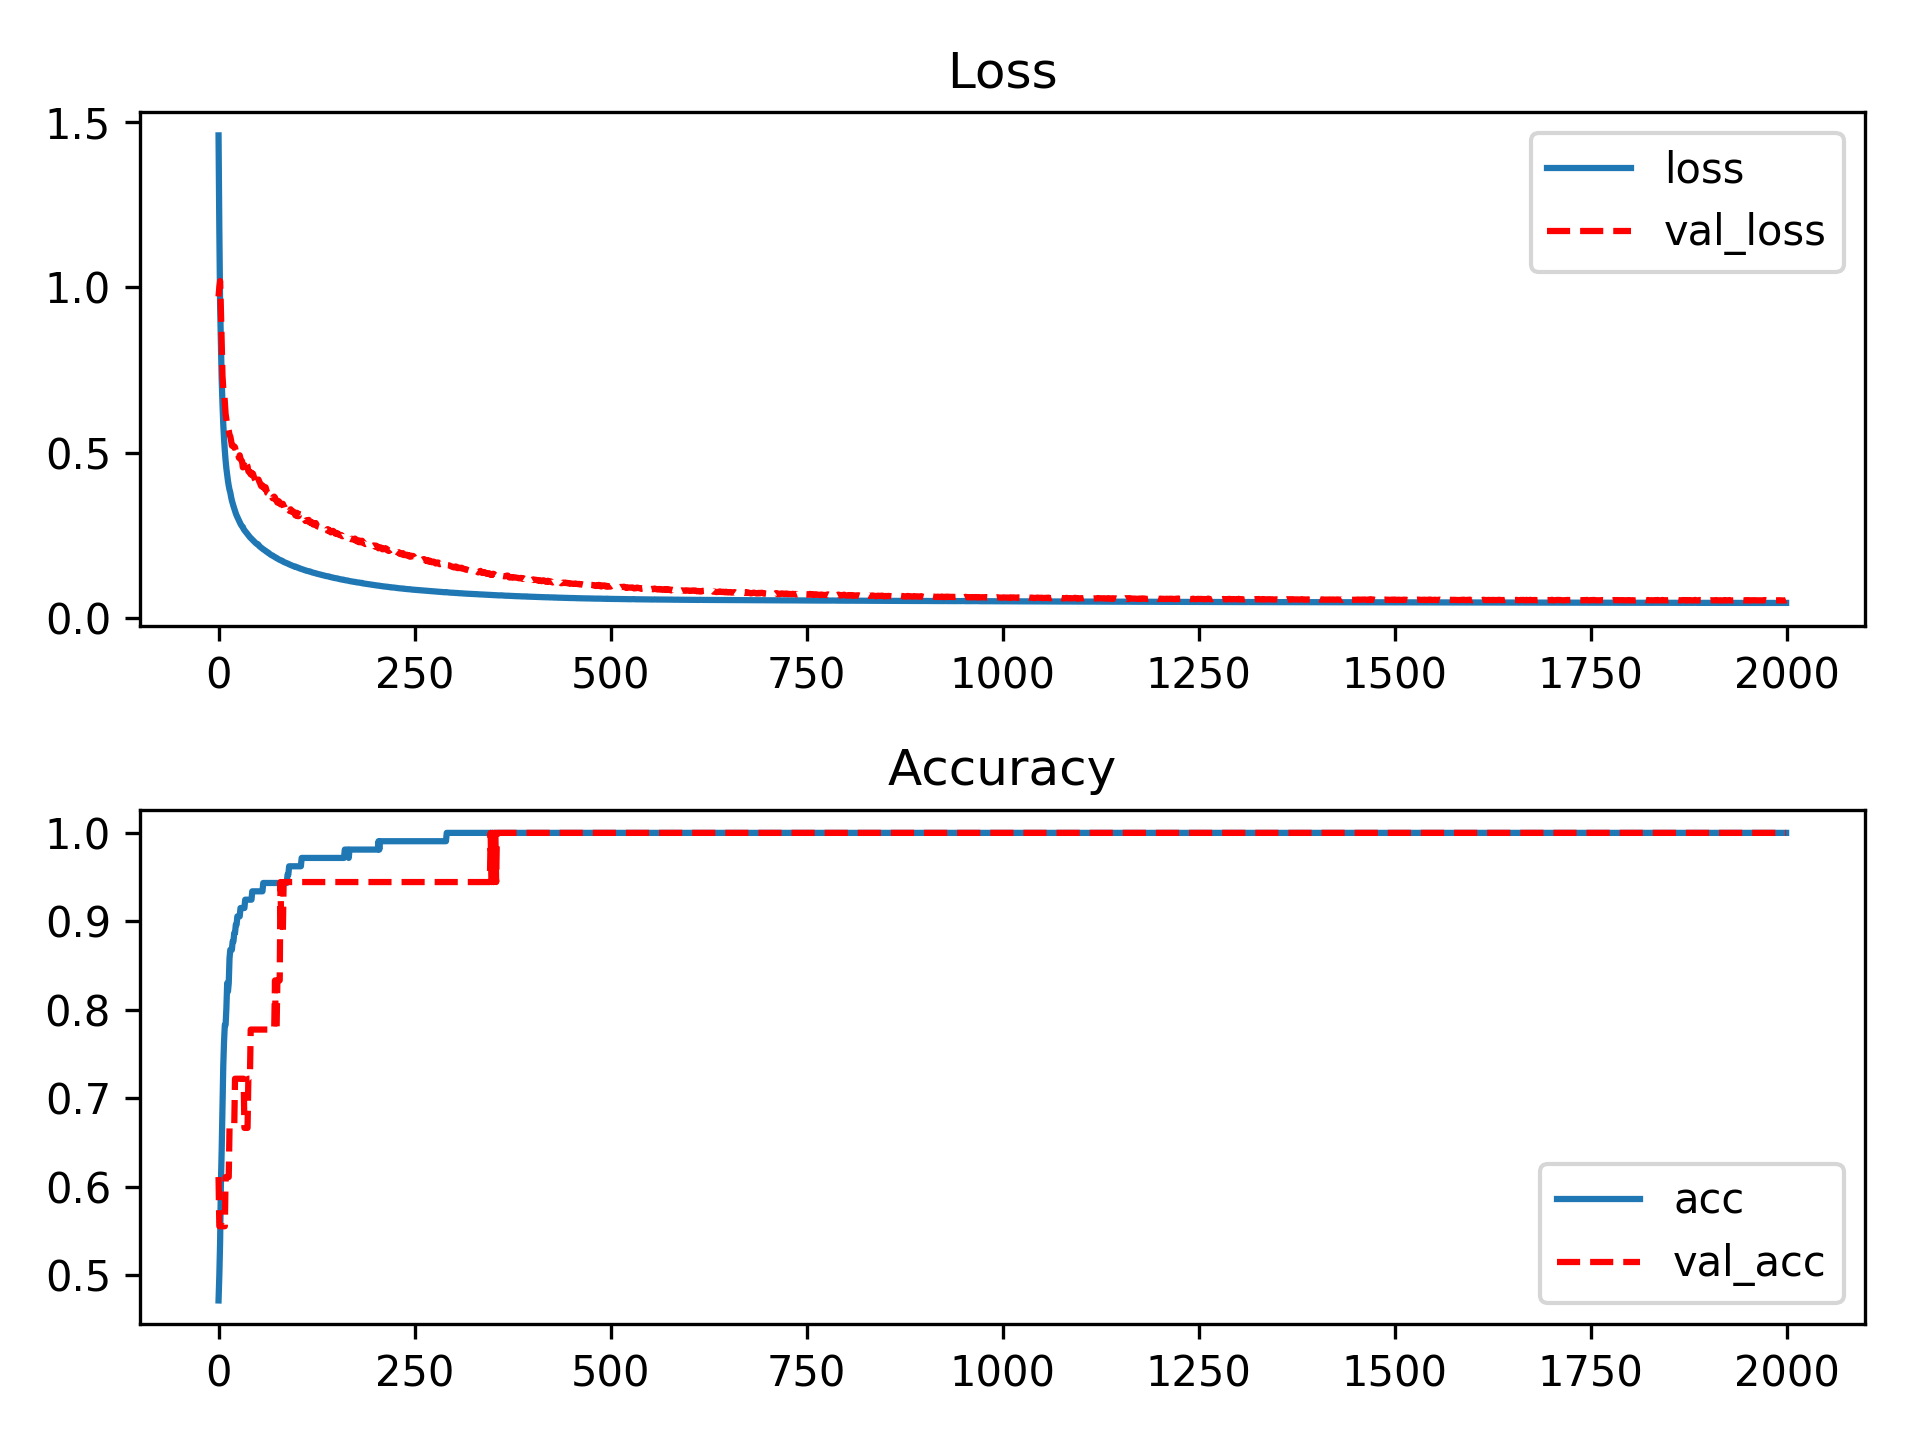
\includegraphics[width=0.8\textwidth]{monks1}
        \caption{Learning curve on MONK 1}
        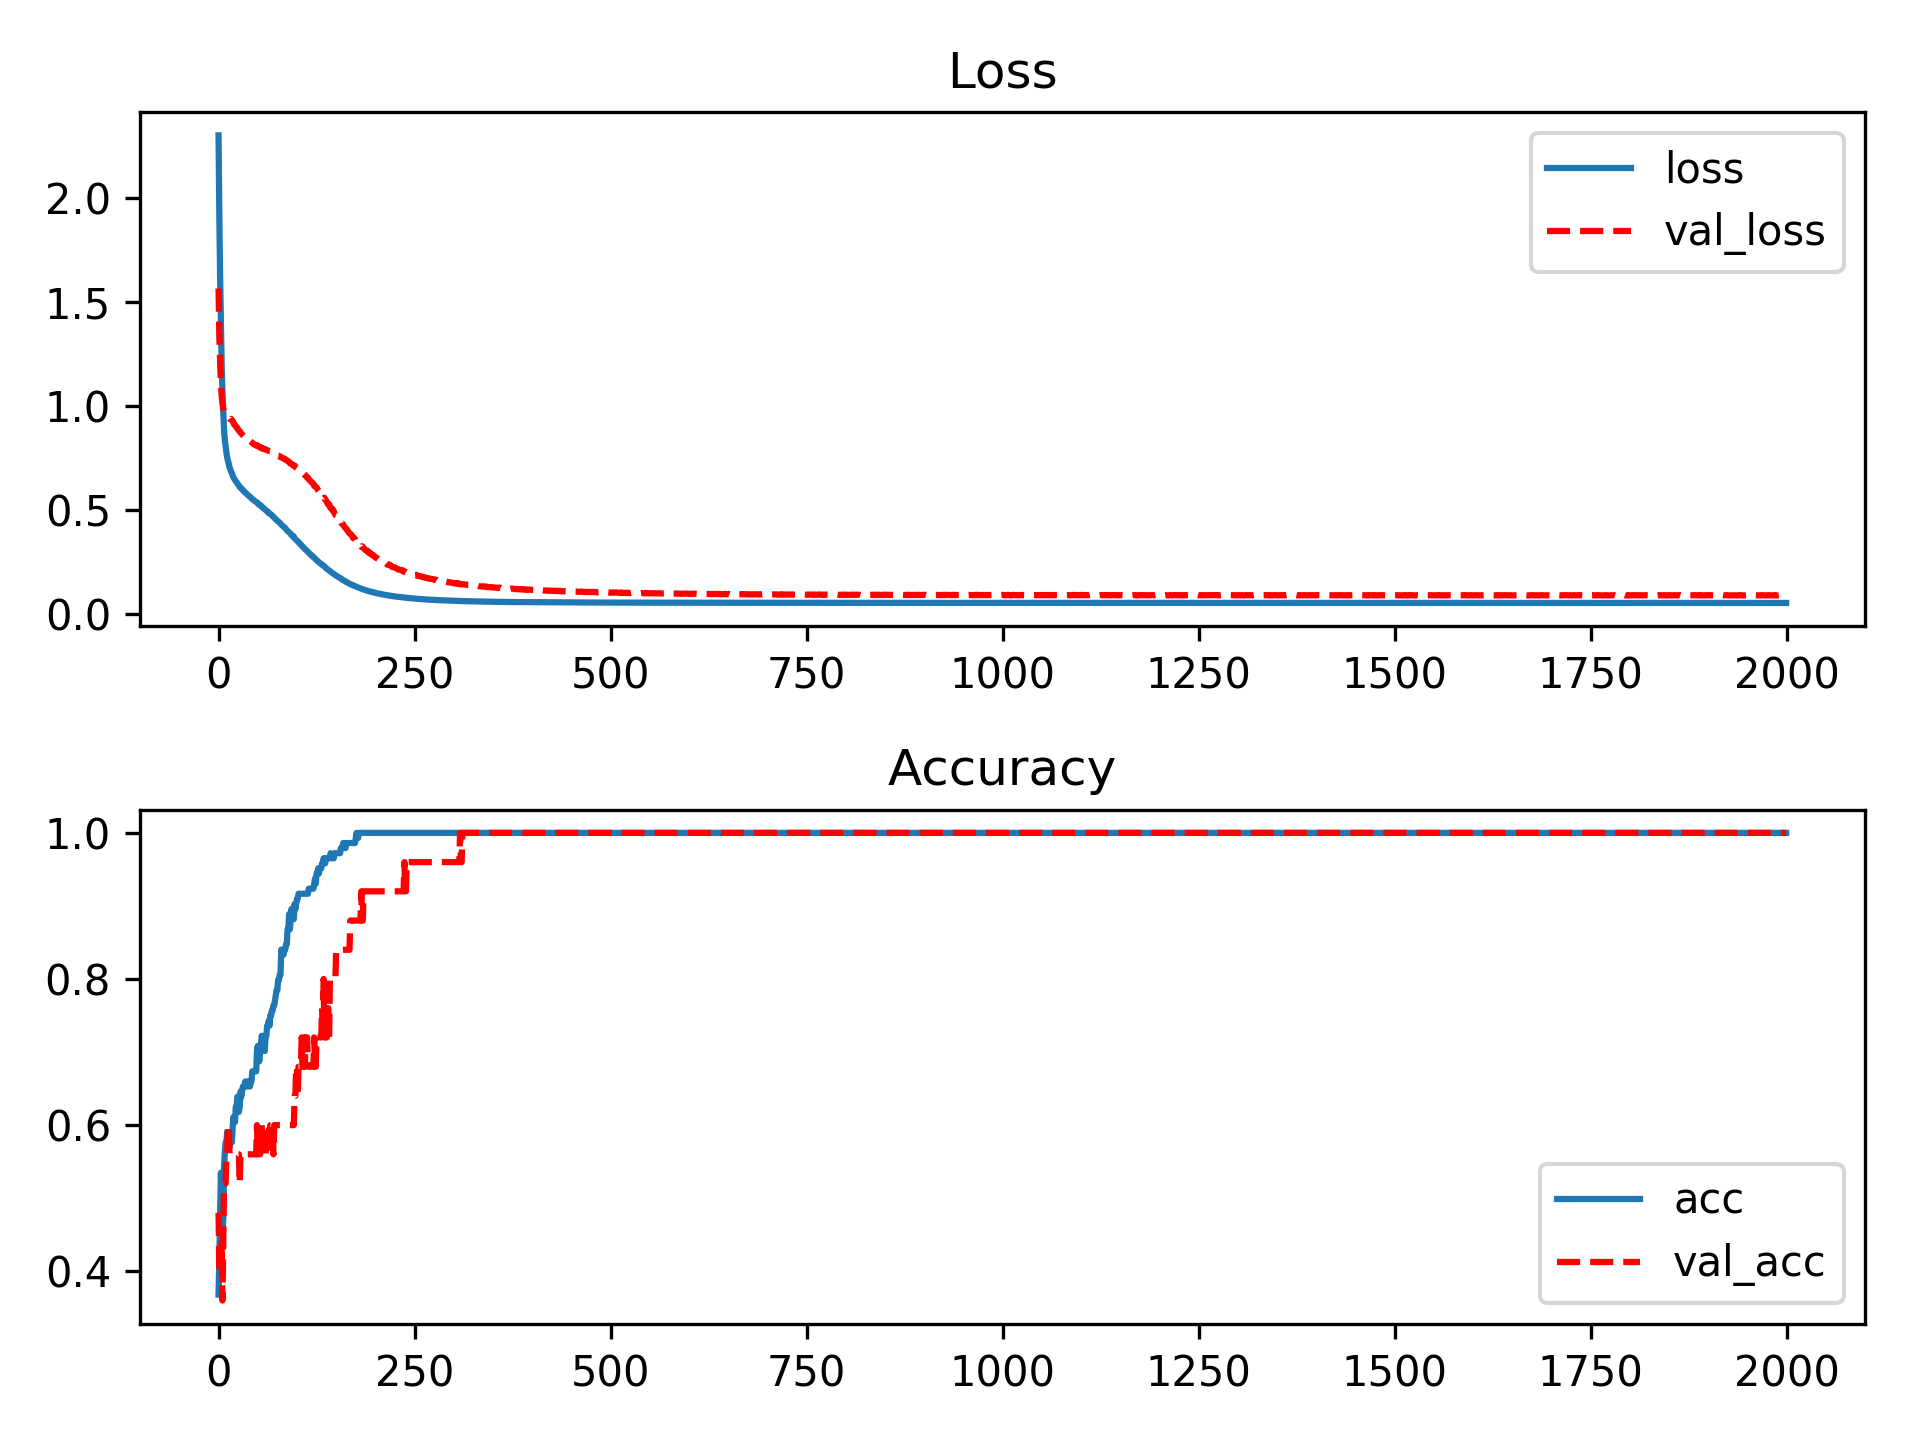
\includegraphics[width=0.8\textwidth]{monks2}
        \caption{Learning curve on MONK 2}
    \end{center}
\end{figure}


\begin{figure}
    \caption{Learning curve on MONK 3 (regularized)}
    \label{fig:monk3}
    \begin{center}
        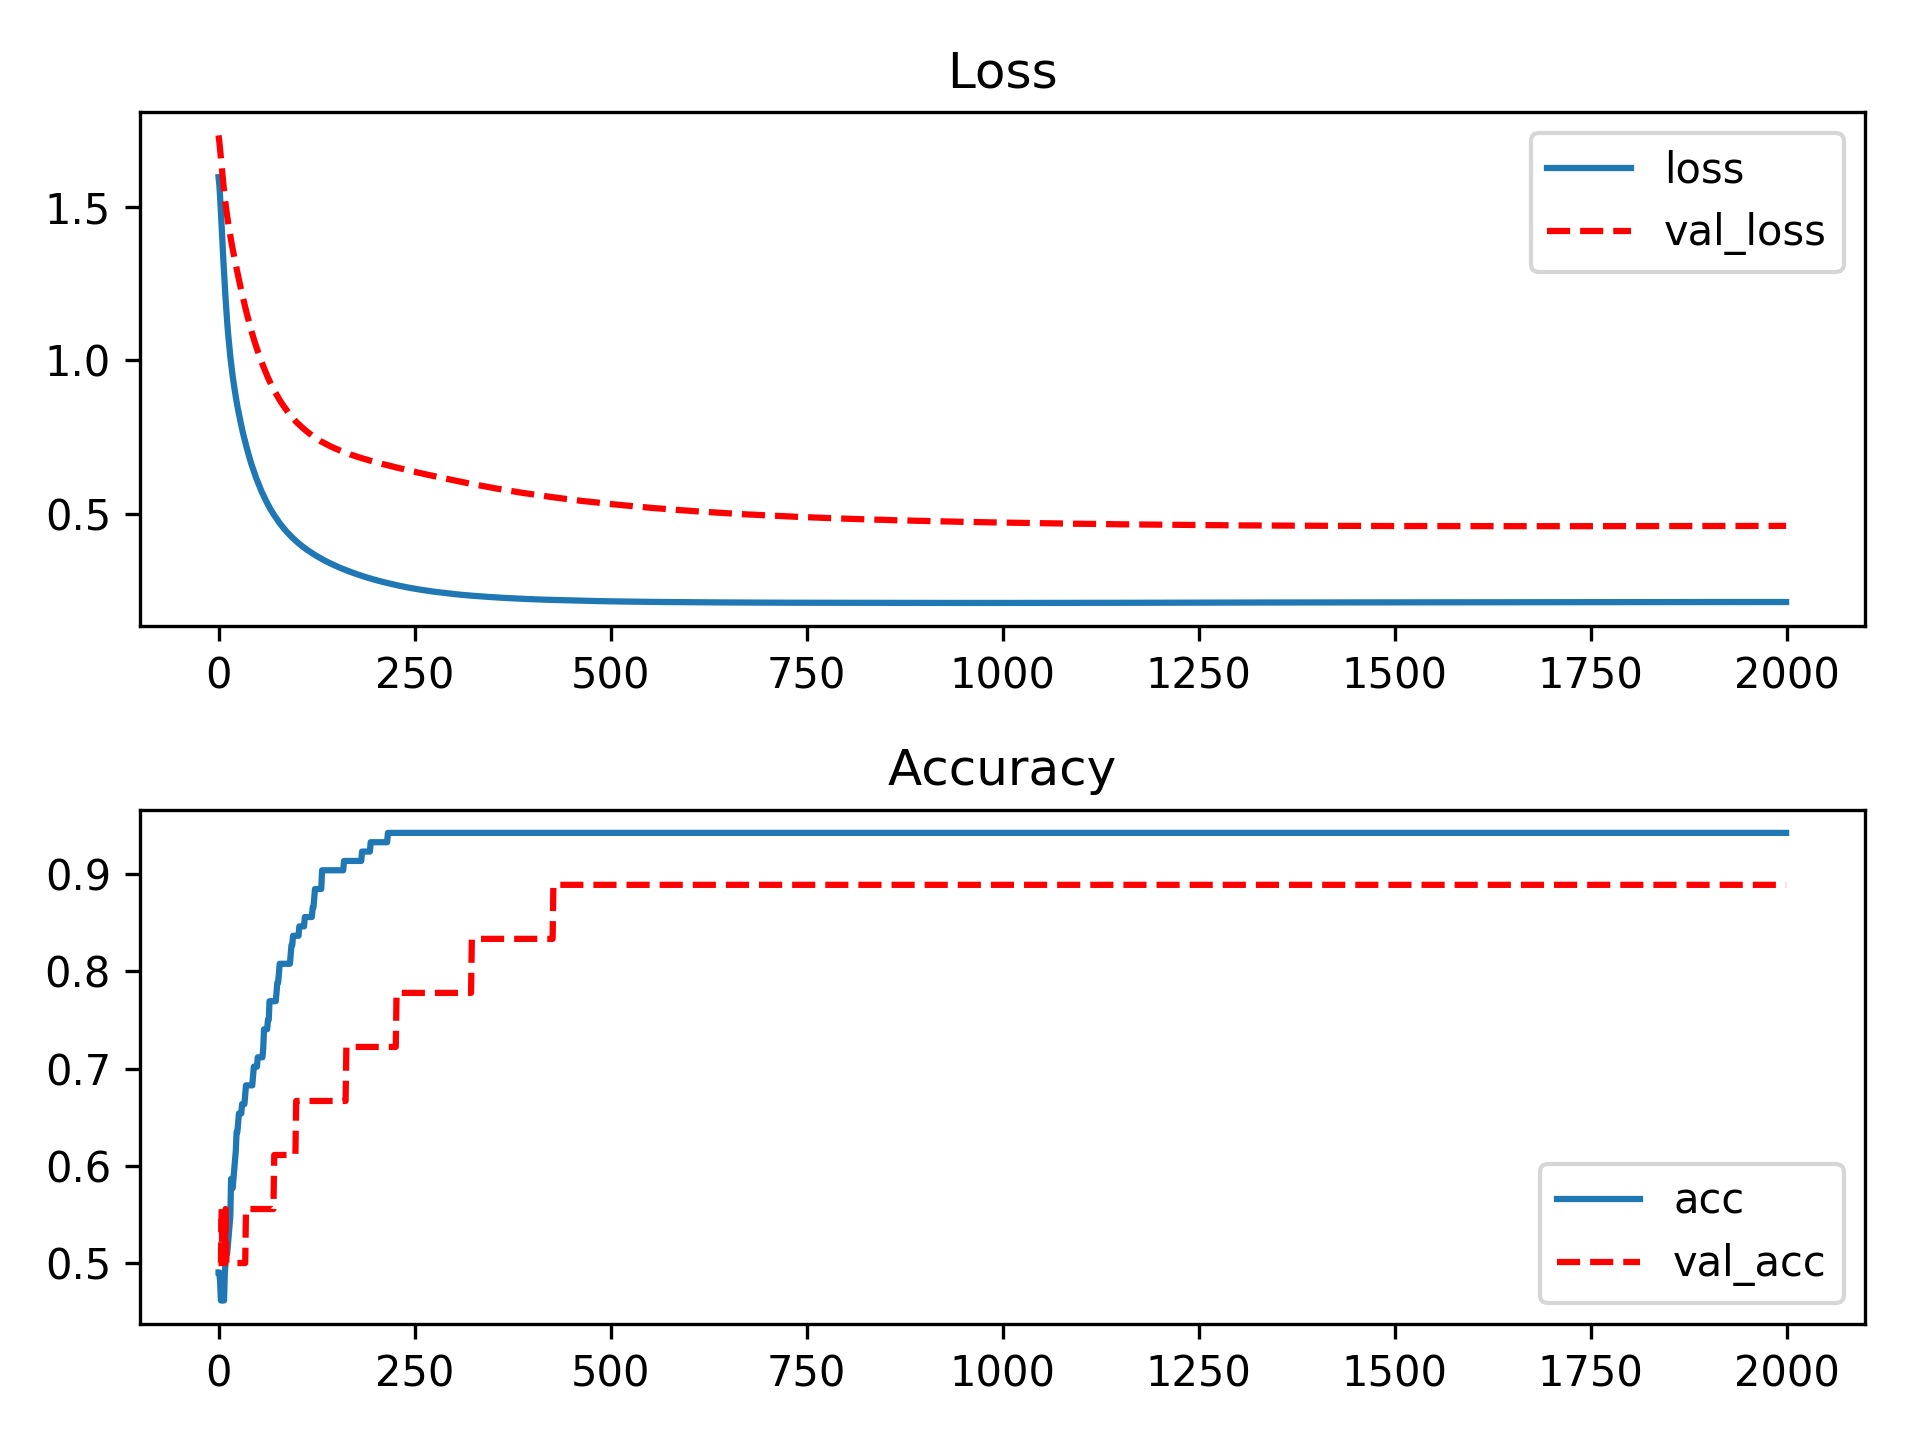
\includegraphics[width=0.8\textwidth]{monks3}
    \end{center}
\end{figure}

\begin{figure}
    \caption{Learning curve on MONK 3 (not regularized)}
    \label{fig:monk3-nr}
    \begin{center}
        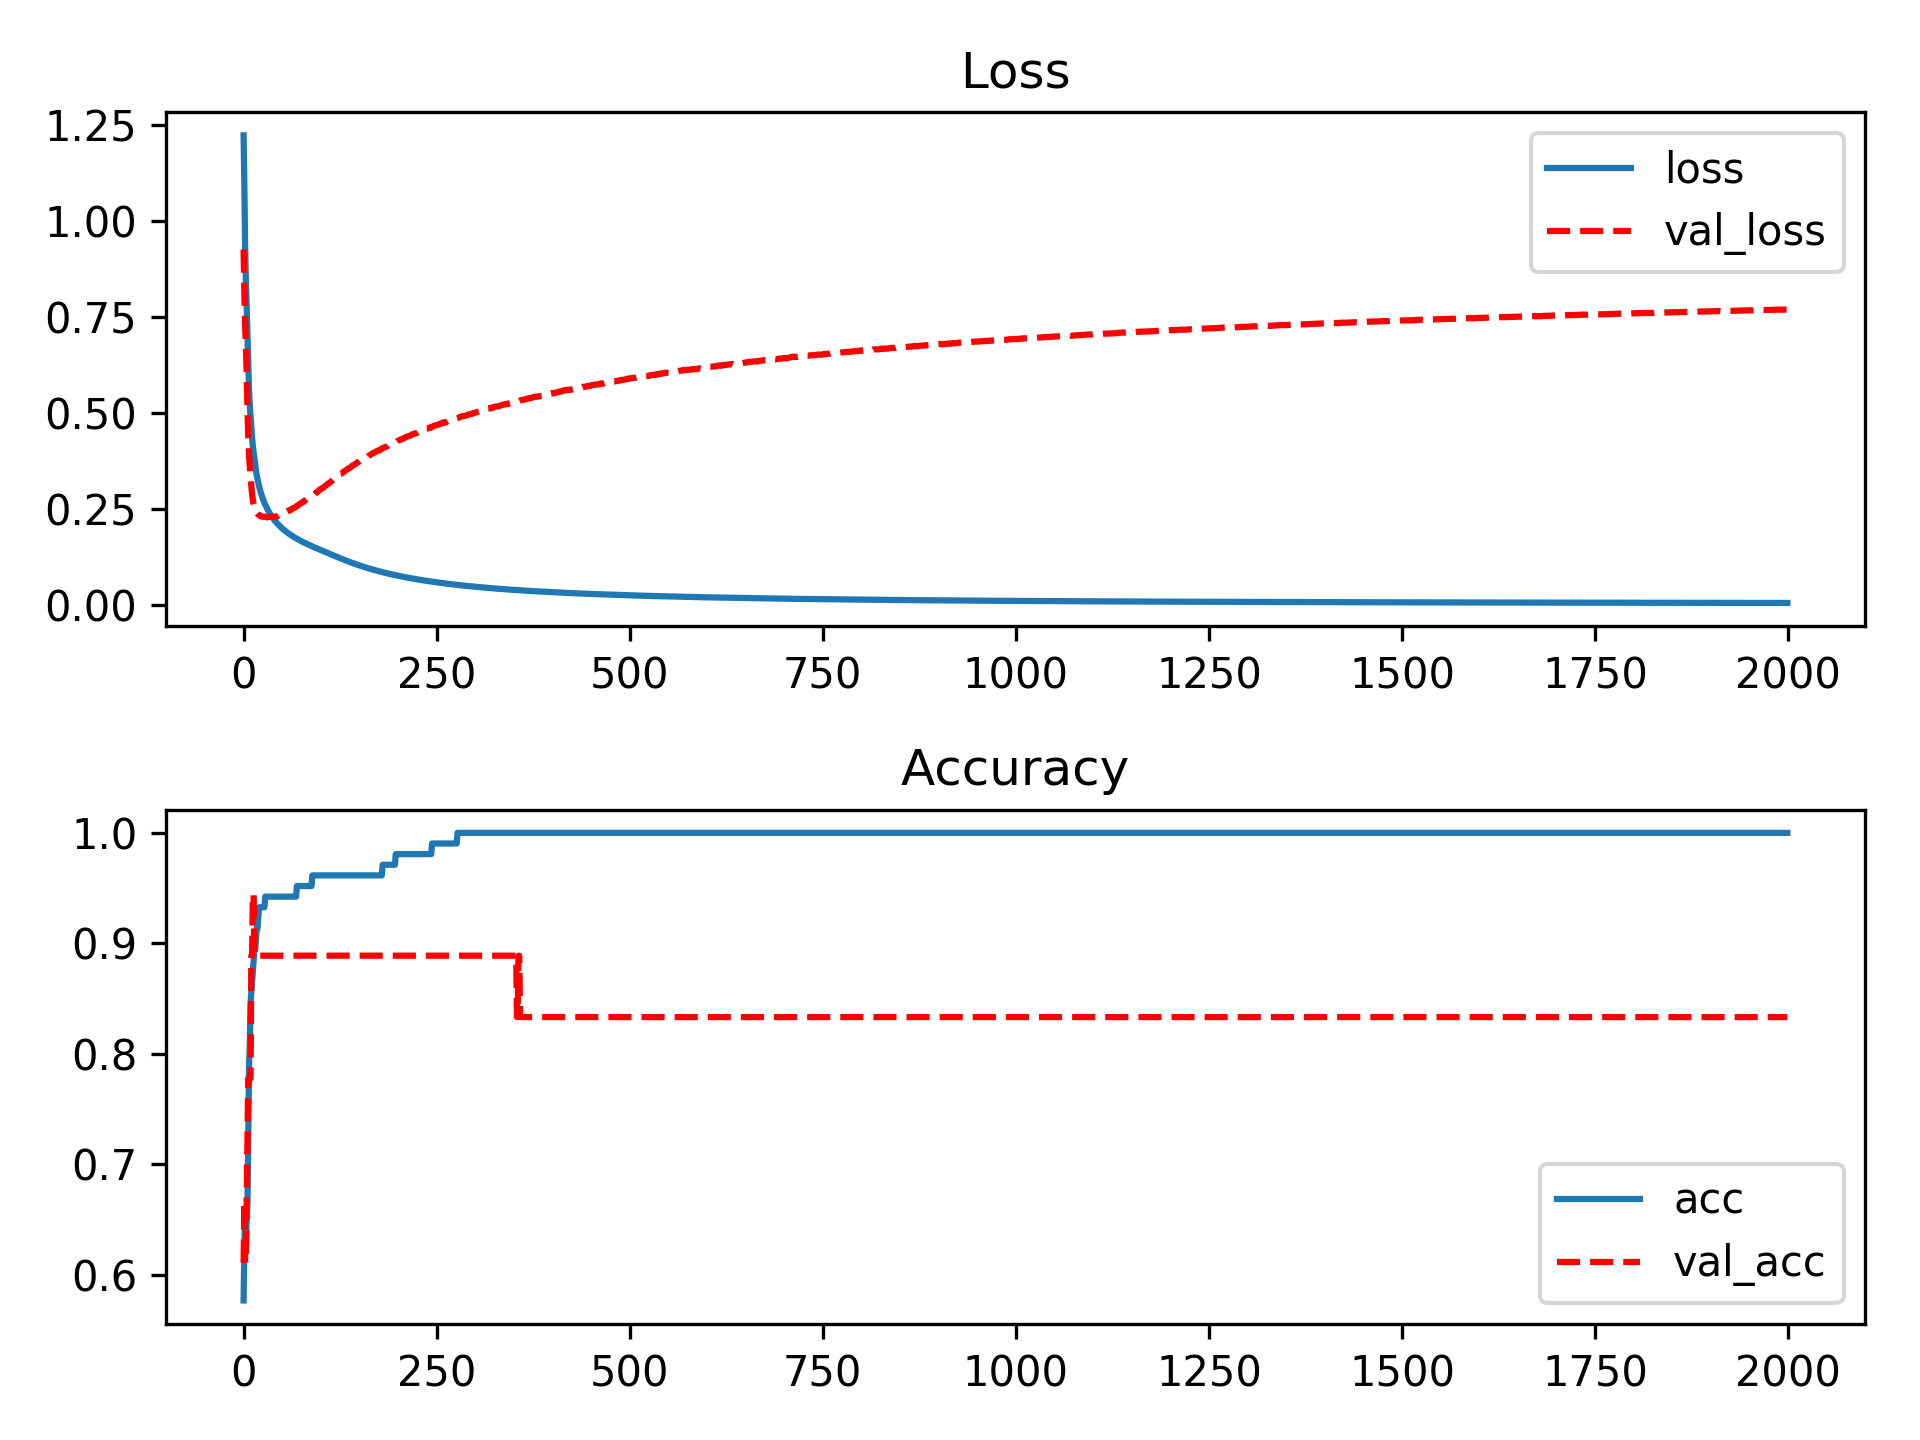
\includegraphics[width=0.8\textwidth]{monks3-nr}
    \end{center}
\end{figure}


We notice that the training loss of MONK 3 (\cref{fig:monk3}) is quite high: this is because the training set has noise, and we are keeping a quite strong regularization.
If instead we remove the regularization, then it overfits as shown in \cref{fig:monk3-nr}

\subsection{CUP results}


%%% Local Variables:
%%% mode: latex
%%% TeX-master: "report"
%%% End:
